
% Beamer document class
\documentclass[xcolor=dvipsnames]{beamer}
% packages
\usepackage[utf8]{inputenc}
%\usepackage{latexsym}
\usepackage{graphicx}
\usepackage{mathptmx}
\usepackage{amsmath}
\usepackage{amsfonts}
\usepackage{amssymb}
\usepackage{amsbsy}
\usepackage{amsthm}
\usepackage{algorithmic}

% Get checkmark logo
\usepackage{pifont}
\newcommand{\cmark}{\ding{51}}
\newcommand{\xmark}{\ding{55}}

% Set VT theme
\usepackage{pgf} % For image/line placement.
% Set a minimal theme with maroon background colors
\setbeamercolor*{palette tertiary}{bg=Maroon}
\setbeamercolor{frametitle}{fg=Black}
\setbeamercolor{section in toc}{fg=Black}
\setbeamercolor{subsection in toc}{fg=Black}
\setbeamercolor{title}{fg=Black}
\setbeamercolor{item}{fg=Black}
\setbeamercolor{block title}{fg=Black,bg=Maroon!20}
\setbeamercolor{caption name}{fg=Black}
% Set the math fonts
\usefonttheme[onlymath]{serif}
\DeclareMathAlphabet{\mathcal}{OMS}{cmsy}{m}{n}
% Create a maroon hline under the frame title
\newcommand{\VThline}{%
\raisebox{-12mm}[0pt][0pt]{%
\begin{pgfpicture}{0mm}{0mm}{0mm}{0mm}
\pgfsetlinewidth{0.28mm}
\color{Maroon}
\pgfline{\pgfpoint{-3mm}{1mm}}{\pgfpoint{10.8cm}{1mm}}
\end{pgfpicture}}}
\setbeamertemplate{headline}{\VThline}
% Add the VT logo to the top right
\newcommand{\VTlogo}{
\vspace*{0.4cm}\hspace*{-3cm}
{
\includegraphics[height=0.5cm]{VPIlogo.png}}}
\setbeamertemplate{sidebar canvas right}{\VTlogo}
% Add page numbers
\setbeamertemplate{footline}[frame number]

% Title Information
\title{Managing Computationally Expensive Blackbox Multiobjective Optimization
Problems with libEnsemble}
\date{May 19, 2020}
\author{Tyler Chang$^1$, Jeffrey Larson$^2$, Layne Watson$^1$, \& Thomas Lux$^1$}
\institute{$^1$ Dept. of Computer Science, Virginia Polytechnic Institute \& State Univ.\\
$^2$ Mathematics and Computer Science Division, Argonne National Laboratory}

\begin{document}

% Make title frame with footnote
\begin{frame}[plain] % plain removes the formatting
\vfill
\titlepage
\vfil % No skip above the logo. If logo is removed, change to \vfill
% Adds logo to bottom of the title page
\centerline{
\includegraphics[height=0.5cm]{VPIlogo.png}}
\end{frame}

% Make ToC
\begin{frame}{Table of Contents}
\tableofcontents
\end{frame}

% VTMOP section
\section{Background in MOPs}
% High-level MOP defn
\begin{frame}{What is a MOP?}
\begin{itemize}
\item The Multiobjective Optimization Problem (MOP) generalizes the Single
Objective (Scalar) Optimization Problem (SOP);
\item The MOP attempts to balance the tradeoff between multiple conflicting
objectives;
\item Whereas the SOP generally has a unique solution, the solution to a MOP
is a {\it set} of {\it Pareto optimal} solutions;
\end{itemize}
\end{frame}
% Pareto/efficient defn
\begin{frame}{The Objective Space and Pareto Front}
\begin{itemize}
\item The solution to a MOP is a set of {\it nondominated} or
{\it Pareto optimal} solutions;
\item $x^*$ is Pareto optimal if for all $x\in\mathcal{X}$, $F(x) \not\leq F(x^*)$;
\begin{center}
\includegraphics[width=0.45\textwidth]{feasible_design.eps}
\includegraphics[width=0.45\textwidth]{convex_pareto.eps}
\end{center}
\end{itemize}
\end{frame}
% Pareto/efficient defn
\begin{frame}{Solving a MOP}
\begin{center}
\begin{tabular}{|ccc|}
\hline
&&\\
&{\large Find a discrete set of approximately}&\\
&{\large nondominated objective points that}&\\
&{\large describes the Pareto front, and the}&\\
&{\large corresponding efficient designs}&\\
&&\\
\hline
\end{tabular}
\end{center}
\end{frame}
% Blackbox problems
\begin{frame}{Expensive Blackbox MOPs}
\begin{center}
{\bf Types of MOPs}\\
\smallskip
{\footnotesize
\begin{tabular}{|c|c|}
\hline
\begin{tabular}{c}
 \\
functions are ``cheap'' to evaluate\\
derivative info is available\\
\\
\end{tabular}
& 
\begin{tabular}{c}
 \\
functions are ``cheap'' to evaluate\\
no derivative info is available\\
\\
\end{tabular}\\
\hline
\begin{tabular}{c}
\\
functions are costly to evaluate\\
derivative info is available\\
\\
\end{tabular}
&
\begin{tabular}{c}
\\
functions are costly to evaluate\\
no derivative info is available\\
\\
\end{tabular}\\
\hline
\end{tabular}
}
\end{center}
\medskip
Focus on bottom right: {\bf expensive blackbox MOPs}!
\end{frame}
%% Common techniques
%\begin{frame}{Common techniques}
%\begin{itemize}
%\item Multiobjective Evolutionary Algorithms
%\begin{itemize}
%\item Requires many function evaluations
%\item Random by nature
%\end{itemize}
%\item Multiobjective Direct Search
%\begin{itemize}
%\item Mainly for biobjective case
%\end{itemize}
%\item Scalarization
%\begin{itemize}
%\item Reduce MOP to SOP using scalarization function
%\item Solve many scalarized subproblems
%\end{itemize}
%\end{itemize}
%\end{frame}
%% Weighted sum
%\begin{frame}{Weighted Sum Method}
%$$
%\min_{x\in\mathcal{X}}\text{ } w^T F(x) \text{, for } w \succeq \Vec{0}
%$$
%\begin{itemize}
%\item For $w > \Vec{0}$, the solution is Pareto optimal
%\item An {\it adaptive weighting scheme} is required
%\item Cannot produce solutions in nonconvex regions of Pareto front\\
%$\qquad\qquad$
%\includegraphics[width=0.5\textwidth]{nonconvex_pareto.eps}
%\end{itemize}
%\end{frame}
%% RSM
%\begin{frame}{The Response Surface Methodology}
%\begin{itemize}
%\item Do an experimental design, use design to fit ``cheap'' surrogate models,
%use surrogates to predict optimal designs
%\item Very economic for blackbox problems
%\item Useful for MOP since the models can be reused for multiple
%scalarizations
%\end{itemize}
%\end{frame}

% Main proposal section
\section{The Algorithm}
% Introducing VTMOP solver...
\begin{frame}{Algorithm Implemented}
Provide a parallel implementation of the multiobjective optimization
algorithm (MOA) proposed by\\
\medskip
{ \small \it Shubhangi Deshpande, et al.
``Multiobjective optimization using an adaptive weighting scheme.''
Optimization Methods and Software 31.1 (2016): 110-133.}\\
\medskip
Combines adaptive weighting scheme, response surface modeling, and trust
region methods
\end{frame}
% Describing Shubhangi's algorithm
\begin{frame}{The Algorithm Outline}
\begin{center}
\includegraphics[width=0.95\textwidth]{algorithm-chart.pdf}
\end{center}
\end{frame}
% Describing Shubhangi's algorithm
\begin{frame}{RSM phases}
\begin{center}
\includegraphics[width=0.95\textwidth]{rsm-chart.png}
\end{center}
\end{frame}
% Describing Shubhangi's algorithm
\begin{frame}{0th iteration}
\begin{center}
\includegraphics[width=0.95\textwidth]{0thit-chart.png}
\end{center}
\end{frame}
% Describing Shubhangi's algorithm
\begin{frame}{Key component}
\begin{center}
\includegraphics[width=0.95\textwidth]{isolated-chart.png}
\end{center}
\end{frame}
% Section on Parallel versions
% Section on Parallel versions
\section{Parallel implementations}
% Source of parallelism
\begin{frame}{Sources of Parallelism}
\begin{enumerate}
\item The function $F$ (left to the user)
\item Iteration complexity (assumed to not offer much improvement)
\item Function evaluations $\leftarrow$ {\bf most important}
\end{enumerate}
\end{frame}
% Describing Shubhangi's algorithm
\begin{frame}{Function evaluations}
\begin{center}
\includegraphics[width=0.95\textwidth]{eval-chart.png}
\end{center}
\end{frame}
% How to use parallelism
\begin{frame}{Parallelizing the original algorithm}
\begin{itemize}
\item Recall that $F$ is being distributed by user
\item Use OpenMP {\it shared memory parallelism}, essentially for achieving
asynchronous behavior
\item Puts burden of distribution on user
\item Better flexibility for real-world HPC systems
\end{itemize}
\medskip\pause
To parallelize function evaluations:
\begin{itemize}
\item Batch of candidates can be trivially evaluated in parallel
\item Instead of using {\tt pVTdirect} from VTDIRECT95 (which uses MPI)
made a modification to the serial code called {\tt bVTdirect} that evaluates
batches of points in parallel using OpenMP
\item For maximal parallelism, replace {\tt bVTdirect} with a Latin hypercube
design, which can be evaluated in parallel
\end{itemize}
\end{frame}
% LibEnsemble
\begin{frame}{libEnsemble}
The {\tt libEnsemble} library is part of the Exascale Computing
Project at Argonne to harness increased levels of concurrency
when distributing large simulations over extreme scale resources
\begin{itemize}
\item Generator function (generates simulations to run)
\item Simulator function (runs simulations, possibly in parallel)
\item Allocator function (decides whether to generate or simulate)
\end{itemize}
\bigskip
\pause
\texttt{VTMOP} is the {\it generator} for {\tt libEnsemble}
\begin{itemize}
\item Each call to the {\it generator} runs a half-iteration and requests
a design exploration (using Latin hypercube) or a batch of candidate evaluations
\item The {\it simulator} evaluates all the requested designs
\item The {\it allocator} waits until all designs are evaluated and then
swithes back to the {\it generator}
\end{itemize}
\end{frame}
% LibEnsemble
\begin{frame}{Integrating with libEnsemble}
\begin{itemize}
\item Want nice big batches that match available resources
\item Use a Latin hypercube search during the search phase
\item Pad out batches of candidates using additional weights
\end{itemize}
\begin{center}
\includegraphics[width=0.7\textwidth]{eval-chart.png}
\end{center}
\end{frame}
% Test functions
\section{Results}
\begin{frame}{Test functions}
\begin{columns}
\begin{column}{.58\textwidth}
\begin{itemize}
\item $F^{(c)}(x) = (\|x - 0.5e^{(1)}\|_2^2, \ldots, \|x - 0.5e^{(p)}\|_2^2)$
\item Convex Pareto front $\Rightarrow$ ``easier'' problem
\end{itemize}
\bigskip\bigskip
\begin{itemize}
\item {\tt DTLZ2} from Deb et al.
\item Concave Pareto front $\Rightarrow$ ``harder'' problem
\end{itemize}
\end{column}
\begin{column}{.4\textwidth}
\bigskip
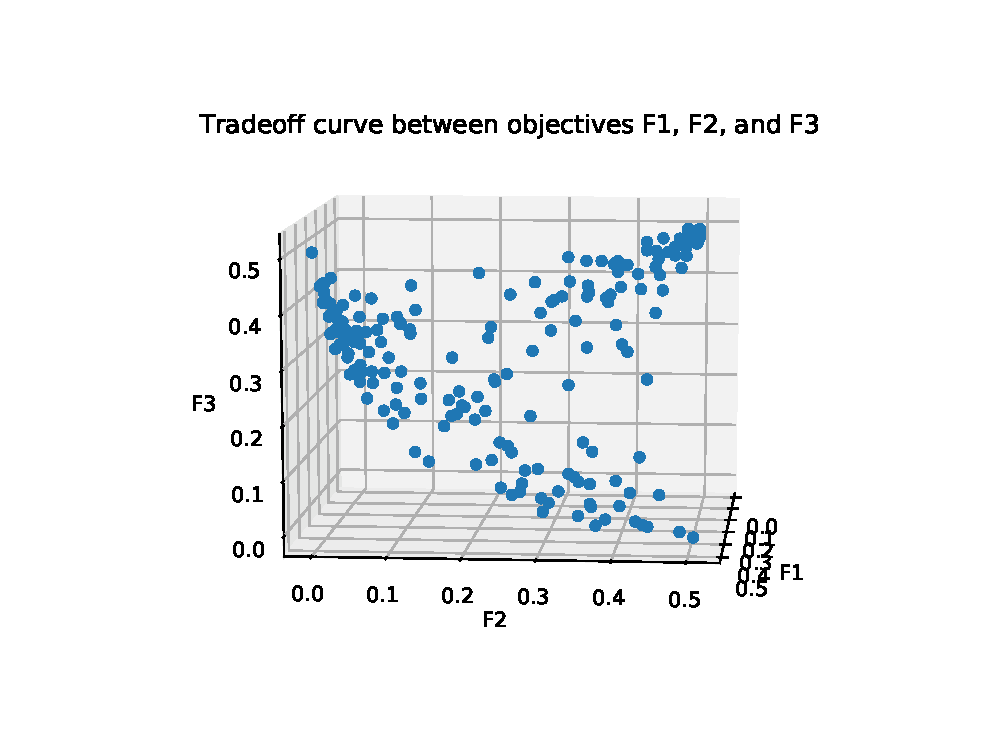
\includegraphics[width=\textwidth]{f_conv_2.eps}\\
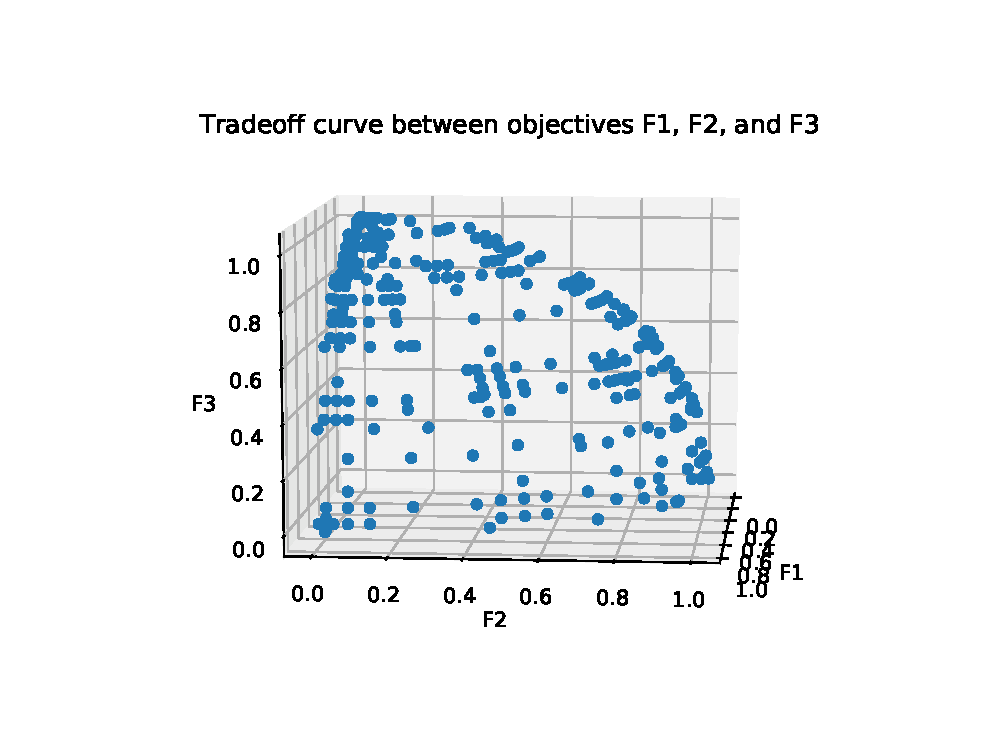
\includegraphics[width=\textwidth]{dtlz2_2.eps}
\end{column}
\end{columns}
\end{frame}
\begin{frame}{Performance metrics}
Evaluating a multiobjective optimization solution is a multiobjective
problem...\\
\medskip
We want:
\begin{enumerate}
\item Many points on the Pareto front (measured by {\it cardinality} of the
solution set)
\item Good convergence of the solution points to the true Pareto front
(measured by RMSE)
\item Even  spacing/good coverage of the solution set
(measured by Delaunay discrepancy, computed with {\tt ScipPy})
\end{enumerate}
\end{frame}
% Performance results
\begin{frame}{Approximation results (2000 evaluations)}
Average (5 runs) number of solutions, RMSE, and Delaunay discrepancy
for $F^{(c)}$ and {\tt DTLZ2} with $d=5$ for VTMOP using {\tt bVTdirect} (DIR),
Latin hypercube search (LH),
and {\tt libEnsemble} (LIBE)\\
\begin{center}
{\small
\begin{tabular}{c|ccc}
Prob/Meth&$p=2$&$p=3$&$p=4$\\
\hline
{$F^c$ / {\tt bVTdir}} & 73, .00100, .207 & 173, .0505, .579 & 288, .101, NA\\
{$F^c$ / {\tt libE1}} & 38, .0115, .180 & 93, .0665, .512 & 171, .117, .689\\
{$F^c$ / {\tt libE2}} & 78, .0127, .158 & 189, .0560, .429 & 283, .104, .551\\
\hline
{{\tt DTLZ2} / {\tt bVTdir}} & 139, .00713, .109 & 354, .0401, .230 & 658, .0443, NA\\
{{\tt DTLZ2} / {\tt libE1}} & 80, .0993, .139 & 264, .167, .458 & 510, .210, .757\\
{{\tt DTLZ2} / {\tt libE2}} & 66, .103, .201 & 258, .175, .691 & 548, .201, .793\\
\end{tabular}
}
\end{center}
NA = Missing values due to {\tt SciPy}'s Delaunay triangulation tool
\end{frame}
% Runtimes
\begin{frame}{Runtime performance (2000 evaluations)}
CPU time / wall time in seconds for DIR, LH, and LIBE versions
with 36 cores \& 1 sec (+ var)/1 core per eval\\
\medskip
\centerline{\small
\begin{tabular}{cc|cccc}
$p$ & Meth & $F_c$ no var & $F_c$ + var & {\tt DTLZ2} no var
& {\tt DTLZ2} + var\\
\hline
& {\tt bVTdir1} & 2008 / 1037 & 2007 / 1039 & 2007 / 1093 & 2004 / 1082\\
& {\tt bVTdir2} & NA / 170 & NA / 239 & NA / 175 & NA / 240\\
$2$ & {\tt libE1} & 2015 / 89 & 2017 / 107 & 2028 / 89 & 2011 / 109\\
& {\tt libE2} & 2051 / 112 & 2070 / 142 & 2060 / 111 & 2064 / 143\\
\hline
& {\tt bVTdir1} & 2012 / 717 & 2012 / 719 & 2021 / 797 & 2018 / 797\\
& {\tt bVTdir2} & NA / 137 & NA / 207 & NA / 165 & NA / 237\\
 $3$ & {\tt libE1} & 2023 / 94 & 2034 / 116 & 2040 / 95 & 2023 / 117\\
& {\tt libE2} & 2077 / 133 & 2066 / 144 & 2054 / 99 & 2057 / 126\\
\hline
& {\tt bVTdir1} & 2026 / 582 & 2029 / 586 & 2177 / 807 & 2149 / 782\\
& {\tt bVTdir2} & NA / 134 & NA / 208 & NA / 280 & NA / 348\\
$4$ & {\tt libE1} & 2042 / 108 & 2045 / 127 & 2176 / 200 & 2201 / 280\\
& {\tt libE2} & 2134 / 190 & 2124 / 186 & 2182 / 227 & 2185 / 257\\
\end{tabular}}
\end{frame}
% show CPU usage plots
\begin{frame}{CPU Usage (36 cores)}
\begin{center}
\includegraphics[width=.4\textwidth]{vtdir_cpu_plt.eps}\\
{\small {\tt bVTdir1} (not suitable for $36$ cores)}\\
\includegraphics[width=.4\textwidth]{libe1_cpu_plt.eps}\hskip 20pt
\includegraphics[width=.4\textwidth]{libe2_cpu_plt.eps}\\
{\small\hskip 10pt {\tt libE1} \hskip 130pt {\tt libE2}}
\end{center}
\end{frame}
\begin{frame}{Questions?}
\tableofcontents
\end{frame}
\end{document}
